

\documentclass[oneside,a4paper,14pt]{extarticle} %размер шрифта 14
\usepackage[T1,T2A]{fontenc}
\usepackage[
a4paper,
letterpaper,
top=2cm,
bottom=2cm,
left=2.5cm,
right=1.5cm
]{geometry}
\usepackage[utf8]{inputenc} %кодировка текста
\usepackage[russian]{babel} %поддержка русского языка
\usepackage{textcomp} %текстовые символы
\usepackage{indentfirst} %корректировка отступов
\usepackage{listings} %для кода !!
\usepackage{float} % для "впихивания" изображений в странницу
\usepackage{xcolor}
\usepackage{enumitem} %для нумерации буквами
\usepackage{graphicx} %работа с изображениям
\usepackage{mwe} % for blindtext and example-image-a in example
\usepackage{wrapfig}
\usepackage{caption}
\usepackage{amsmath}  % для формул и символов
\usepackage{amsfonts}
\usepackage{amsthm}
\usepackage{graphicx}
\usepackage[all]{xy}
\usepackage[breaklinks]{hyperref}
\usepackage{xurl}

%%размеркегляузаголоковразделов
\usepackage{titlesec}
\titleformat{\section}
{\normalsize\bfseries}
{\thesection} {1em}{}
\titleformat{\subsection}
{\normalsize\bfseries}
{\thesubsection} {1em}{}
\titleformat{\subsubsection}
{\normalsize\bfseries}
{\thesubsection} {1em}{}

\renewcommand\baselinestretch{1.33}\normalsize % межстрочный интервал
\setlength{\parindent}{1.25cm}
\usepackage{indentfirst}

\lstset{
	language=C,
	basicstyle=\ttfamily\small,
	keywordstyle=\color{blue},
	commentstyle=\color{green!60!black},
	stringstyle=\color{red},
	numbers=left,
	numberstyle=\tiny\color{gray},
	frame=single,
	breaklines=true,
	showstringspaces=false,
	tabsize=2,
	inputencoding=utf8,
	extendedchars=true
}

\begin{document}
	\newpage\thispagestyle{empty}
	\begin{center}
		МИНИСТЕРСТВО НАУКИ И ВЫСШЕГО ОБРАЗОВАНИЯ\\
		РОССИЙСКОЙ ФЕДЕРАЦИИ
		ФЕДЕРАЛЬНОЕ ГОСУДАРСТВЕННОЕ БЮДЖЕТНОЕ\\
		ОБРАЗОВАТЕЛЬНОЕ
		УЧРЕЖДЕНИЕ ВЫСШЕГО ОБРАЗОВАНИЯ\\
		«ВЯТСКИЙ ГОСУДАРСТВЕННЫЙ УНИВЕРСИТЕТ»\\
		Институт математики и информационных систем\\
		Факультет автоматики и вычислительной техники\\
		Кафедра электронных вычислительных машин
	\end{center}
	\vspace{20mm}
	
	\begin{center}
		Отчёт по лабораторной работе №4\\
		по дисциплине\\
		<<Алгоритмы и структуры данных>>\\
	\end{center}
	\vspace{48mm}
	
	\noindent
	Выполнил студент гр. ИВТб-1303-06-00 \hfill \rule[-0,5mm]{30mm}{0.15mm}\,/Шубин В.Ю./
	\newline
	Проверил заведующий кафедрой ЭВМ \hfill \rule[-0,5mm]{30mm}{0.15mm}\,/Долженкова М.Л./
	
	\vfill
	\begin{center}
		Киров\\
		2026
	\end{center}
	
	\newpage
	% \thispagestyle{empty}
	
	\section*{Цель работы:}
	Отточить навыки решения задач в условиях ограниченного времени.
	
	\section*{Вводные}
	Для выполнения данной лабораторной работы был выбран Codeforces Round 2231 (Div. 2). 
	\url{https://codeforces.com/contest/2231}
	
	\section*{Описание процесса решения}
	Было выбрано и запущено виртуальное соревнование.
	Открыл задачу A - Составьте массив \url{https://codeforces.com/contest/2227/problem/A}.
	В данной задаче требуется создать массив a, где 1 <=a[i]<=2*n и каждый элемент
	встречается в нем только один раз. Еще, суммы соседних элементов (a[i] + a[i+1],
	a[i+1] + a[i+2] и т.д.) также должны быть уникальны и не встречаться в массиве.
	Я заметил, что если брать только нечетные числа, то решение оказывается очень простым.
	Идем по диапазону и берем числа 1, 3, 5 и т.д.. Таким образом, суммы будут четными, 
	что уже исключает их появление в основном массиве. Так как мы берем числа по 
	возрастанию, каждая сумма будет больше предыдущей, что также исключает повторы.
	На эту задачу ушло немало времени, я очень долго не мог понять условие. Я считаю что это либо
	плохая формулировка, либо плохой перевод.
	
	
	\begin{lstlisting}[caption={Решение задачи A - Составьте массив}]
		t = int(input())
		for _ in range(t):
			n = int(input())
			res = [2 * i + 1 for i in range(n)]
		print(*res)
	\end{lstlisting}
	\url{https://codeforces.com/contest/2231/submission/377054993}
	\newpage
	
	В задаче B. Очередная задача на сортировку (\url{https://codeforces.com/contest/2231/problem/B}) требуется 
	отсортировать данный массив по неубыванию, применив операцию: выбрать число k и прибавить его к каждому 
	элементу выбранной подпоследовательности массива. Эту операцию можно применить лишь один раз. Вывести
	ответ "YES"/"NO" если сортировка таким способом возможна или нет. Если элемент больше следующего, то мы
	прибавляем к меньшему k. Значит, минимально возможное значение k должно быть не меньше разности таких элементов.
	Если массив нельзя отсортировать с минимальным k, то сделать это с бОльшим k тоже невозможно. Также можно было 
	добавить в начало кода проверку, отсортирован ли уже массив (если да - вывод YES и break), но я забыл, когда
	отправлял решение.
	
	\begin{lstlisting}[caption={Решение задачи B. Очередная задача на сортировку}]
		t = int(input())
		for _ in range(t):
		
			n = int(input())
			a = list(map(int, input().split()))
			
			L = 0
			for i in range(n - 1):
			if a[i] > a[i + 1]:
				L = max(L, a[i] - a[i + 1])
			
			prev = a[0]
			for i in range(1, n):
				if a[i] >= prev:
					prev = a[i]
				elif a[i] + L >= prev:
					prev = a[i] + L
				else:
					print("NO")
					break
				else:
					print("YES")
	\end{lstlisting}
	\url{https://codeforces.com/contest/2227/submission/377058481} \\
	
	
	
	Следующую задачу C - Бурундучонок Тео и равенство (\url{https://codeforces.com/contest/2231/problem/C}) я не успел
	решить из-за времени: Во-первых, я не мог придумать код который не превысит время компиляции в 2000 мс, 
	а во-вторых, мои 2 часа для прохождения соревнования подошли к концу. По итогу мой код оказался вроде бы верным
	и рабочим, но не подходящим для больших объемов данных. В данной задаче нужно найти минимальное количество шагов, 
	за которое можно уравнять все элементы массива. Есть две операции - деление четного элемента на 2 и +1 к нечетному.
	За каждый шаг можно выполнить только одну операцию и только для одного элемента. Можно подсчитать статистику путей
	и кол-ва шагов, за которое каждый элемент доходит до значения 1, и в конце выбрать то значение, до которого смогли дойти
	все элементы с минимальным кол-вом шагов. Алгоритм слишком сложный, поэтому было превышение по времени выполнения.
	
	
	\begin{lstlisting}[caption={Решение задачи C - Бурундучонок Тео и равенство}]
		t = int(input())
		for _ in range(t):
			n = int(input())
			a = input().split()
			counts = {}
			for x in a:
				x = int(x)
				counts[x] = counts.get(x, 0) + 1
			freq = {}
			cost = {}
			
			for x, cnt in counts.items():
				curr = x
				d = 0
				seen = set()
				while curr not in seen:
					seen.add(curr)
					if curr not in freq:
						freq[curr] = cnt
						cost[curr] = d * cnt
					else:
						freq[curr] += cnt
						cost[curr] += d * cnt
					d += 1
					if curr % 2 == 0:
						curr //= 2
					else:
						curr += 1
			
			ans = -1
			for k, v in freq.items():
				if v == n:
					if ans == -1 or cost[k] < ans:
						ans = cost[k]
			print(ans)
	\end{lstlisting}
	\url{https://codeforces.com/contest/2227/submission/377059342}
	
	\subsection*{Скриншот отправленных решений}
	\begin{figure}[H]
		\centering
		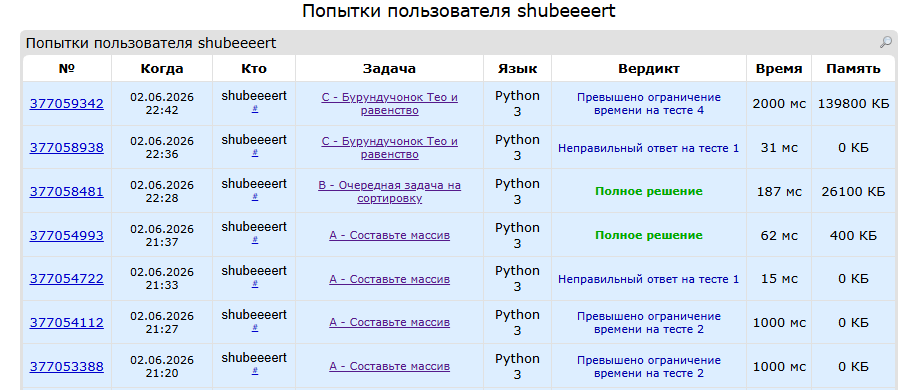
\includegraphics[width=\textwidth, height=\textheight, keepaspectratio]{result.png}
	\end{figure}
	
	\section*{Выводы}
	Проанализировав своё участие в соревновании я пришёл к выводу, что мне нужно больше времени для обдумывания поставленных условий,
	подбора подходящего алгоритма и проверки кода на ошибки для получения качественного результата. \\
	\newline
	\indent
	Вообщем, я считаю, что мне просто надо учиться решать задачки, но это приходит с опытом.
	
	
	
\end{document}